\chapter{Curve Fitting}

\section{Introduction}

In this exercise, you will learn about curve fitting with Scientific Python
function {\tt curve{\_}fit}.  Given a function to fit $f(x;p)$, with p
representing any number of parameters, and a set of measurements $y_i$ and points $x_i$,
the {\tt curve{\_}fit} function determines the best fit parameters by
minimizing:
\begin{displaymath}
\chi^2 = \sum_i \frac{(f(x_i;p) - y_i) ^2}{\sigma_i^2}.
\end{displaymath}
If the uncertainties $\sigma_i$ are not specified, the function
assumes $\sigma_i = 1$, and still finds the correct minimum
if the actual uncertainties are identical to one another.

\section{Fitting a Straight Line}

\begin{figure}[htbp]
\begin{center}
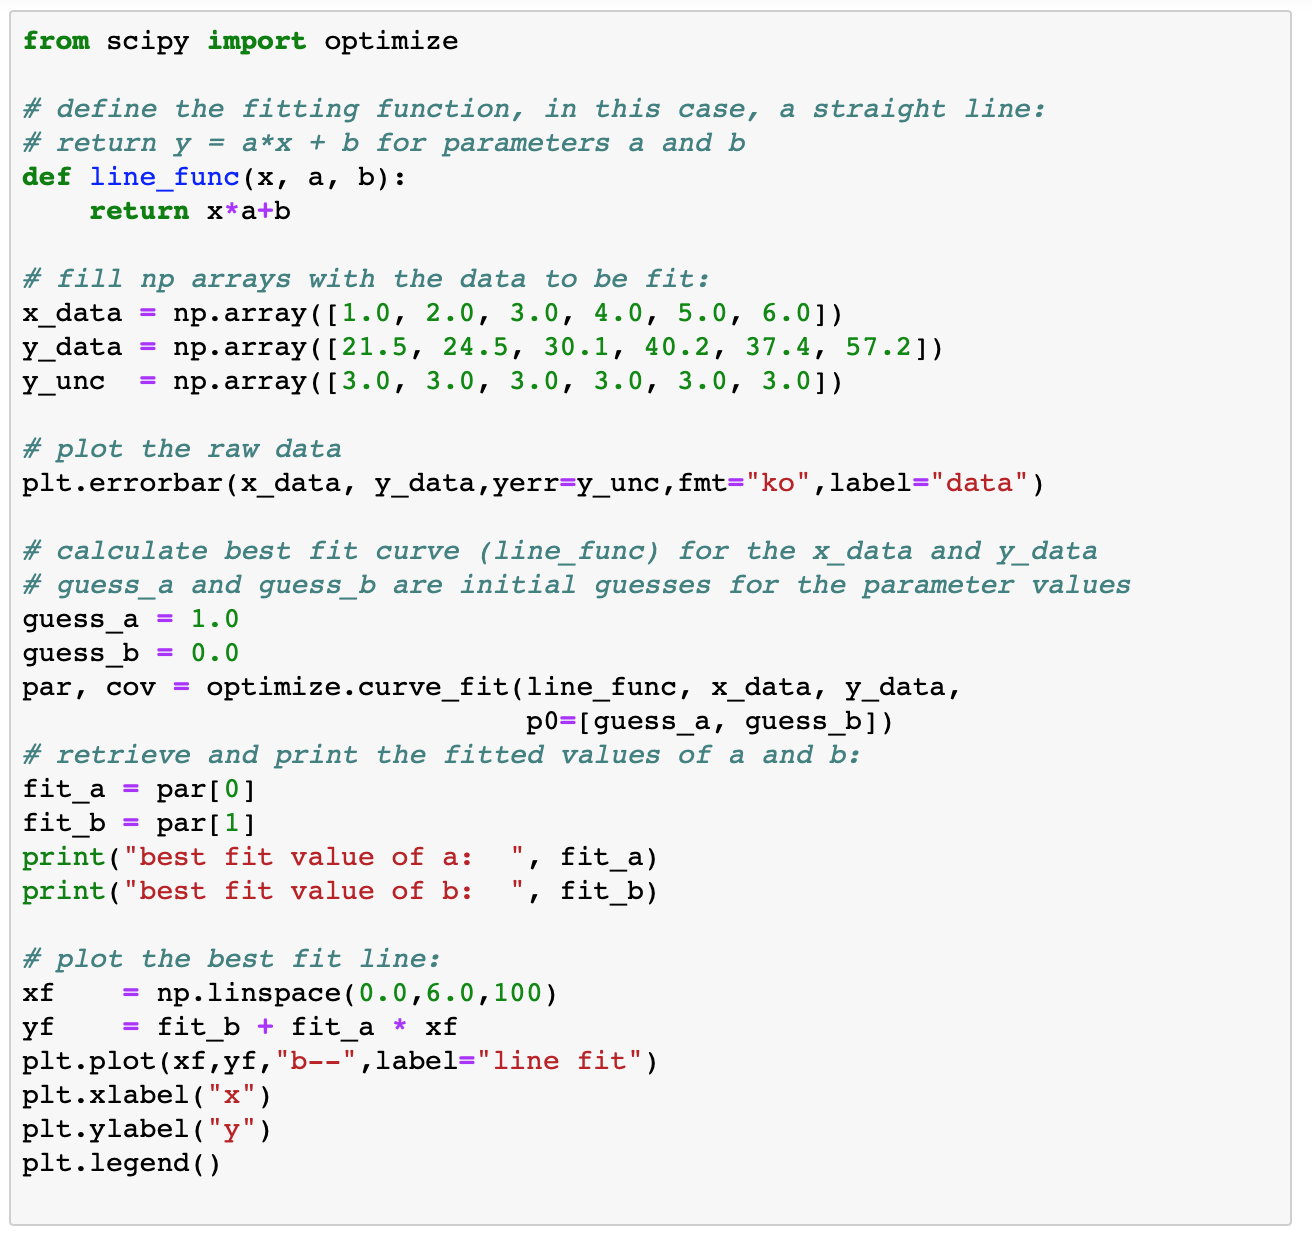
\includegraphics[width=1.0\textwidth]{figs/fitting/fit_code.png} \\
\caption{Example fitting data to straight line.}
\label{fig:fiteg}
\end{center}
\end{figure}

\begin{figure}[htbp]
\begin{center}
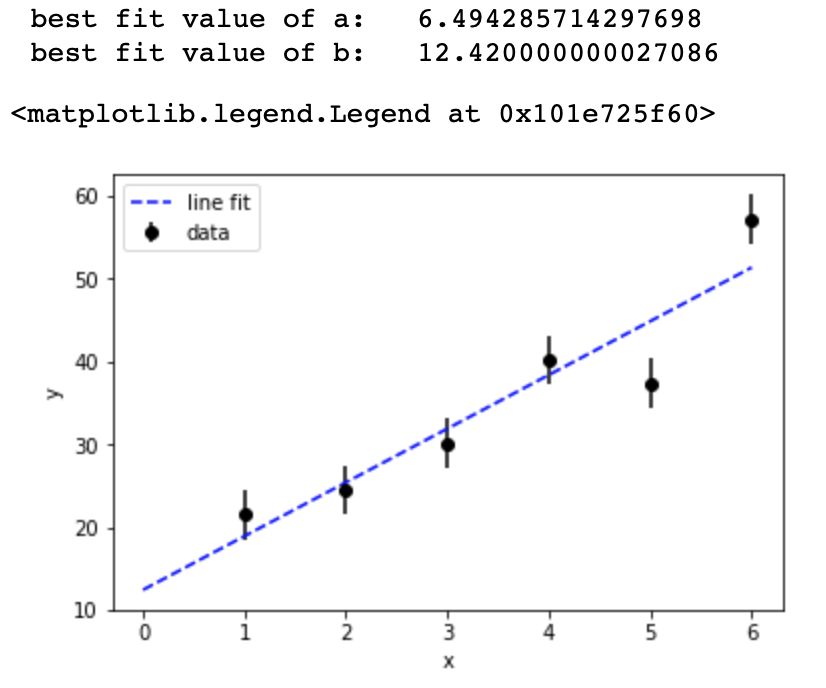
\includegraphics[width=0.65\textwidth]{figs/fitting/fit_out.png} \\
\caption{Output of example fit.}
\label{fig:fiteg}
\end{center}
\end{figure}

An example using Scientific Pythons {\tt curve{\_}fit} function to fit
a straight line to data is shown in Fig.~\ref{fig:fiteg}.  A block of 
code defining the function we wish to fit, in this case, a straight
line, is defined as a function:
\begin{verbatim}
     def line_func(x, a, b):
         return a*x + b
\end{verbatim}
In this case, the function requires three parameters (in the computer
science sense) the x data in a numpy array as function parameter x,
the slope as function parameter a, and the intercept as function
parameter b.  When called, the function returns the x data multiplied
by the value a, with the value b added.  We don't directly call this
function, but in principle, it could be called like:
\begin{verbatim}
    y_data = line_func(x_data, 2.0, 0.0)
\end{verbatim}
to create a numpy array {\tt y{\_}data} constructed from {\tt
  x{\_}data} with slope 2 and intercept 0.

The next section filling numpy arrays containing the data, and
plotting it with error bars should be familiar by now.  The fit itself
is performed by the line:
\begin{verbatim}
par, cov = optimize.curve_fit(line_func, x_data, y_data, p0=[guess_a, guess_b])
\end{verbatim}
This performs a fit of the function {\tt line{\_}func} defined above
to the $x$ and $y$ data contained in the arrays {\tt x{\_}data} and
{\tt y{\_}data}.  Numerical fits generally find the local minimum,
which is not necessarily the global minimum of interest.  It is
important therefore, especially for complicated fits, to provide an
initial guess near the expected fit values.  These are provided to the
optional, named, function parameter {\tt p0}, which is set to the
python list {\tt [guess{\_}a, guess{\_}b]} which contains our initial guesses for
the fit parameters $a$ and $b$.  The function performs a least-squares
fit to find the best values of $a$ and $b$ which are returned as the
numpy array {\tt par}.  The function also returns the covariance
matrix as the numpy array {\tt cov}.

The remaining code simply uses the best fit values to plot the fitted
function as a dashed line.  Numerical fits are fickle.  Even if you
are only interested in the fitted value, you should always plot the
best-fit function and compare the results to your data as in important
check for your work.

\begin{table}
\caption{Sample data for straight line fit.}
\label{tbl:linesamp}
\begin{center}
\begin{tabular}{ll}
$x$ & $y \pm \sigma_y$ \\
1.0  & $15.9 \pm 3.0$ \\
2.0  & $23.6 \pm 3.0$ \\
3.0  & $33.9 \pm 3.0$ \\
4.0  & $39.7 \pm 3.0$ \\
5.0  & $45.0 \pm 10.0$ \\
6.0  & $32.4 \pm 20.0$ \\
\end{tabular}
\end{center}
\end{table}

\begin{figure}[htbp]
\begin{center}
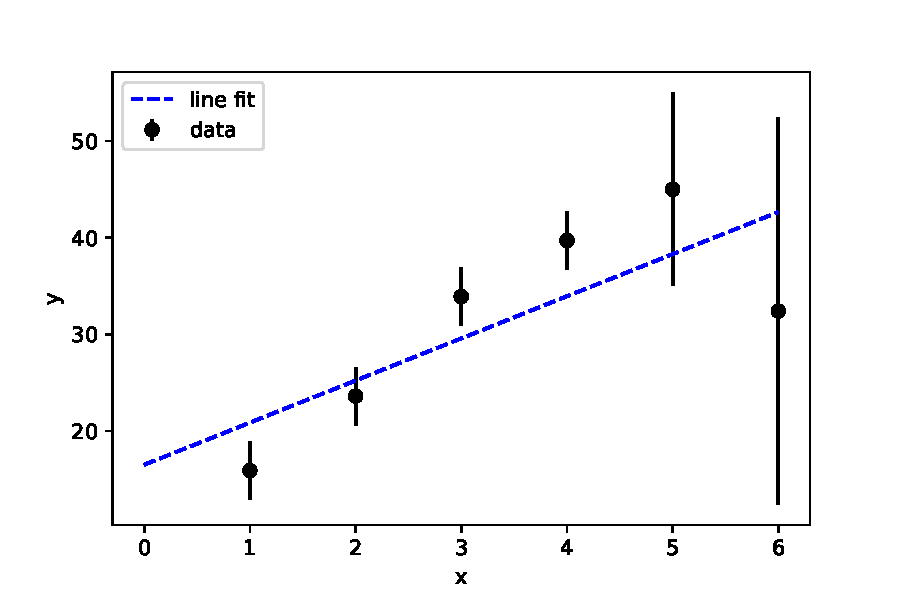
\includegraphics[width=0.65\textwidth]{figs/fitting/bias.pdf} 
\caption{This linear fit is biased by the failure to properly account for uncertainties.}
\label{fig:fitbias}
\end{center}
\end{figure}

Produce {\bf Plot 1} by applying code like that of Fig.~\ref{fig:fiteg}
to the data in Table~\ref{tbl:linesamp} to reproduce the plot in
Fig.~\ref{fig:fitbias}.  

Notice that the last two data points have larger uncertainties than
the other data points.  However, the call to the {curve{\_}fit}
function does not provide the parameter uncertainties, and so the
function assumes that they all have the value $1$.  In this case,
since the uncertainties are not in fact all the same, the function
does not find the correct minimum.  The answer is clearly biased
toward the poorly measured points, because the function gives these
points the same weight as all of the other points.

Look-up the {\tt curve{\_}fit} function and the optional parameter
{\tt sigma}.  For {\bf Plot 2}, provide the correct uncertainties to
the fit.  You should observe that the fit results is no longer biased,
and more closely tracks the well constrained left side of the plot.

\section{Fitting a Sine Curve}

In this section, you will fit the sample data to a sine function:
\begin{displaymath}
 y = A \, \sin( k x). 
\end{displaymath}
Use the following sample data:\\
\begin{center}
\begin{tabular}{|ll| ll|ll|}
\hline
$x$ & $y$ & $x$ & $y$ & $x$ & $y$\\
\hline
0  & 5.3    & 4  & -9.7   & 8  & 15.7  \\
1  & 15.0   & 5  & -17.4  & 9  & 18.5  \\
2  & 19.2   & 6  & -20.5  & 10 & 8.6   \\
3  & 6.8    & 7  &  2.1   & &  \\
\hline
\end{tabular}
\end{center}
Assume the uncertainty is the same for each $y$ value: $\sigma_i = 2$.
For {\bf Plot 3}, plot the data including error bars and the best-fit
sine wave.  





















